% Chapter Template

\chapter{SAFT-$\gamma$ Mie Force Field} % Main chapter title

\label{ChapterX} % Change X to a consecutive number; for referencing this chapter elsewhere, use \ref{ChapterX}

%----------------------------------------------------------------------------------------
%	SECTION 1
%----------------------------------------------------------------------------------------

\section{SAFT-VR Mie}

The SAFT-VR Mie equation of state \cite{lafitte2013} is the basis for the SAFT-$\gamma$ Mie coarse grained force field \cite{avendano2011}. This EoS was initially developed to describe chain molecule formed from fused Mie segments using the Mie attractive and repulsive potential. The Mie potential is a type of generalized Lennard-Jones potential that can be used to describe explicitly repulsive interactions of different hardness/softness and attractive interactions of different ranges, and is given by:
\begin{equation}
U_{Mie}(r) = \epsilon\frac{\lambda_r}{\lambda_r - \lambda_a} \left(\frac{\lambda_r}{\lambda_a} \right)^{\left( \frac{\lambda_a}{\lambda_r - \lambda_a} \right)}
\left[ \left(\frac{\sigma}{r} \right)^{\lambda_r} - \left(\frac{\sigma}{r} \right)^{\lambda_a} \right]
\label{eqn:miepotential}
\end{equation}
where $\epsilon$ is the potential well depth, $\sigma$ is the segment diameter, r is the distance between the spherical segments, $\lambda_r$ is the repulsive exponent and $\lambda_s$ is the attractive exponent. This equation uses the \citeonline{bh1976} high perturbation expansion of the Helmholtz free energy up to third order in addition to a improved expression for the  radial distribution function (RDF) of Mie monomers at contact to obtain a equation capable to give an accurate theoretical description of the vapor-liquid equilibria and second derivative properties \cite{lafitte2013}. For a non-associating fluid, the Helmholtz free energy is:
\begin{equation}
\frac{A}{N\kappa_{b}T} = a = a^{IDEAL} + a^{MONO} + a^{CHAIN}
\label{eqn:miehelm}
\end{equation}

%	SUBSECTION 1
%-----------------------------------
\subsection{Ideal Contribution}

The ideal contribution for a mixture is given by:
\begin{equation}
a^{IDEAL} = \sum_{i=1}^{N_{c}} x_{i}\ln{(\rho_{i}{\Lambda_{i}}^3)} -1
\label{eqn:aideal}
\end{equation}
where $x_{i}=N_{i}/N$ is the molar fraction of component i, $\rho_{i}=N_{i}/V$ is the number density, $N_{i}$ is the number of molecules of each component and $\Lambda_{i}^3$ is de Broglie wavelength. 
%-----------------------------------
%	SUBSECTION 2
%-----------------------------------

\subsection{Monomer Contribution}
The monomer contribution describes the interactions between Mie segments and can be expressed for a mixture as:
\begin{equation}
a^{MONO} = \left(\sum_{i=1}^{N_{c}} x_{i}m_{s,i} \right)a^{M}
\label{eqn:amonomer}
\end{equation}
In the equation above, $m_{s,i}$ is the number of spherical segments making up the molecule i and $a^{M}$  is the monomer dimensionless Helmholtz free energy and it is expressed as a third order perturbation expansion in the inverse temperature \cite{bh1976}:
\begin{equation}
a^{M} = a^{HS}+\beta{a_{1}}+\beta{a_{2}}^2+\beta{a_{3}}^3 
\label{eqn:aM}
\end{equation}
where $\beta=\kappa_{b}T$ and $a^{HS}$ is the hard-sphere dimensionless Helmholtz free energy for a mixture :
\begin{equation}
a^{HS} = \frac{6}{\pi\rho_{s}}\left[\left(\frac{\zeta^3_2}{\zeta^2_3}-\zeta_0 \right)\ln(1-\zeta_3)+\frac{3\zeta_{1}\zeta_{2}}{1-\zeta_3}+ \frac{\zeta^3_2}{\zeta_{3}(1-\zeta_3)^2}\right]
\label{eqn:hs}
\end{equation}
The $\rho_{s}=\rho\sum_{i}^{N_c} x_{i}m{s,i}$ is the total number density of spherical segments and $\zeta_l$ are the moments of the number density:
\begin{equation}
\zeta_l = \frac{\pi\rho_s}{6}\left(\sum_{i=1}^{N_c} x_{s,i}d^l_{ii} \right), l = 0,1,2,3
\label{eqn:zetal}
\end{equation}
where $x_{s,i}$ is the mole fraction of the segments and is related through the mole fraction of component i ($x_i$) by:
\begin{equation}
x_{s,i} = \frac{m_{s,i}x_i}{\sum_{k=1}^{N_c} m_{s,k}x_{k} }
\label{eqn:xsi}
\end{equation}
The effective hard-sphere diameter $d_{ii}$ for the segments is:
\begin{equation}
d_{ii} =\int_{0}^{\sigma_{ii}} ( 1 - \exp(-\beta U^{Mie}_{ii}(r)) ) dr
\label{eqn:diameter}
\end{equation}
The integral in Eq. \eqref{eqn:diameter} is normally obtained by means of Gauss-Legendre with a 5-point quadrature \cite{papa2014}. The detailing of the terms of Eq. \eqref{eqn:amonomer} can be found in \citeonline{lafitte2013}.
\subsection{Chain Contribution}
The chain formation of $m_{s}$ tangentially bonded Mie segments contribution is based on the first-order pertubation theory (TPT1)  \cite{papa2014} and can be expressed as:
\begin{equation}
a^{CHAIN} =-\sum_{i=1}^{N_{c}} x_{i}(m_{s,i} - 1)\ln(g_{ii}^{Mie}(\sigma_{ii}))
\label{eqn:achain}
\end{equation}
The $g_{ij}^{Mie}(\sigma_{ij})$ term correspond to the value of the radial distribution function (RDF) of the hypothetical Mie system evaluated at the effective diameter and can be obtained with the perturbation expansion:
\begin{equation}
g_{ij}^{Mie}(\sigma_{ij}) =g_{d,ij}^{HS}(\sigma_{ij})\exp[\beta\epsilon \nicefrac{g_{1,ij}(\sigma_{ij})}{g_{d,ij}^{HS}(\sigma_{ij})} + (\beta\epsilon)^2 \nicefrac{g_{2,ij}(\sigma_{ij})}{g_{d,ij}^{HS}(\sigma_{ij})}]
\label{eqn:achain}
\end{equation}
The terms in the equations above are explicitly exposed in the original article \cite{lafitte2013}. 
\subsection{Ring Contribution}
There are two forms for the Helmholtz free energy for rings formed from $m_{s}$ tangentially bonded segments in the literature. The first one  \cite{lafitte2012} considered that the difference between a chain and a ring molecule is that the latter one has one more bond that is connecting the first segment to the last. With this assumption, the Eq. \eqref{eqn:achain} becomes:
\begin{equation}
a^{RING} =-\sum_{i=1}^{N_{c}} x_{i}m_{s,i}\ln(g_{ii}^{Mie}(\sigma_{ii}))
\label{eqn:aringlafitte}
\end{equation}
According to \citeonline{lafitte2012}, Eq. \eqref{eqn:aringlafitte} needs an additional parametrization with molecular simulation data so the EoS can  be used in molecular simulations, but this procedure is not the necessary for ring molecules. Recently \citeonline{muller2017} tried to correct this inconsistency developing the ring free energy based on the work of \citeonline{muller1993} whom obtained rigorous expressions for molecular geometries of rings of $m_s=3$ for hard fluids. The final expression for the dimensionless Helmholtz free energy is:
\begin{equation}
a^{RING} =-\sum_{i=1}^{N_{c}} x_{i}(m_{s,i}-1+\chi_{i}\eta_{i})\ln(g_{ii}^{Mie}(\sigma_{ii}))
\label{eqn:aringmuller}
\end{equation}
where $\eta_{i}=m_{s,i}\rho_{i}\sigma_{ii}^{3}/6$ is the packing fraction and $\chi_{i}$ is a parameter which depends on $m_{s,i}$ and the geometry of the ring of each component i. For a value of $\chi=0$ Eq. \eqref{eqn:aringmuller} is equal to Eq. \eqref{eqn:achain} and $\chi=1.3827$ corresponds to a hard sphere system of triangles. \citeonline{muller2017} also calculated values of $\zeta$ for the Saft-VR Mie EoS for the values of $m_{s}=3,m_{s}=4,m_{s}=5,m_{s}=7$ with pseudo-experimental data from molecular dynamics (MD) for a defined pure fluid. The values of $\chi$ estimated can be seen in the figure below:
\begin{figure}[th]
\centering
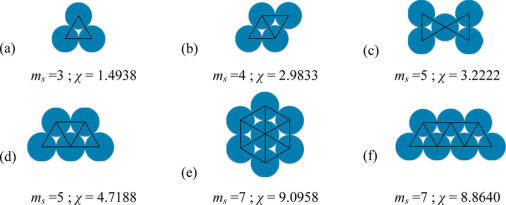
\includegraphics[scale=0.8]{Figures/mullergeo.jpg}
\caption{Values for parameter $\chi$ according to the ring geometry \cite{muller2017}}
\label{fig:ringqsi}
\end{figure}
\subsection{Combining rules for the intermolecular potential parameters}
\citeonline{lafitte2013} also suggested mixing rules for the potential parameters:
\begin{equation}
\sigma_{ij} =\frac{\sigma{ii}+\sigma{jj}}{2}
\label{eqn:sigmamix}
\end{equation}
\begin{equation}
\lambda_{k,ij} -3 =\sqrt{(\lambda_{k,ii}-3)(\lambda{k,jj}-3)} , k=r,a
\label{eqn:lambdamix}
\end{equation}
\begin{equation}
\epsilon_{ij} =(1-k_{ij})\frac{\sqrt{\sigma_{ii}^{3}\sigma_{jj}^{3}}}{\sigma_{ij}^{3}}\sqrt{\epsilon_{ii}\epsilon_{jj}}
\label{eqn:epsmix}
\end{equation}
The $k_{ij}$ is a binary interaction parameter to account the mixture behavior. This parameter can also be fitted to experimental data.
%----------------------------------------------------------------------------------------
%	SECTION 2
%----------------------------------------------------------------------------------------

\section{Parameter Estimation for the SAFT-$\gamma$ Mie Force Field}

